\documentclass{standalone}
\usepackage{tikz}
\usepackage{pgf}
% \usepackage{luatex85}
\usetikzlibrary{graphs, shapes}
% \usetikzlibrary{graphdrawing}
% \usegdlibrary{layered}


\pgfdeclareradialshading{ballshading}{\pgfpoint{-12bp}{10bp}}
{color(0bp)=(yellow!15!white);
color(5bp)=(yellow!15!white);
color(6bp)=(yellow);
% color(18bp)=(yellow!70!black);
% color(25bp)=(yellow!50!black);
color(50bp)=(black)
}

\pgfdeclareradialshading{ballshading1}{\pgfpoint{-12bp}{10bp}}
{color(0bp)=(orange!15!white);
color(5bp)=(orange!15!white);
color(6bp)=(orange);
% color(18bp)=(orange!70!black);
% color(25bp)=(orange!50!black);
color(50bp)=(black)
}

\pgfdeclareradialshading{ballshading2}{\pgfpoint{-12bp}{10bp}}
{color(0bp)=(red!15!white);
color(5bp)=(red!15!white);
color(6bp)=(red);
% color(18bp)=(red!70!black);
% color(25bp)=(red!50!black);
color(50bp)=(black)
}

% \tikzstyle{type0} = [circle, shading=ball, ball color=yellow, draw=yellow!50!red, thick, label=0]
\tikzstyle{0} = [shading=ballshading, circle, draw=green!70!red, thick, label={center:0}, minimum size=5mm]
\tikzstyle{1} = [shading=ballshading1,circle, draw=yellow!50!red, thick, label={center:1}, minimum size=5mm]
\tikzstyle{2} = [shading=ballshading2,circle, draw=black!90!red, thick, label={center:2}, minimum size=5mm]
% \tikzstyle{2} = [circle, fill=white!90!red, draw=yellow!50!red, thick, label=2]
\begin{document}
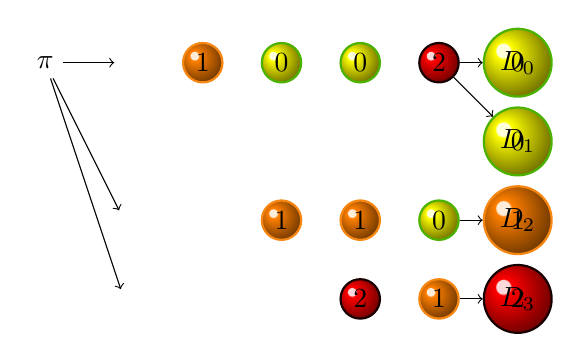
\begin{tikzpicture}[
  % -!-,
  % every node/.style={radius=3pt},
  % layered layout,
  centered
  ]
  % \node (0-1) at (10,0) {hey};
   % \foreach \x [count = \i] in {2,...,5}
     % \node (0-\x) [left of=0-\i] {\x};
  \graph [trie, grow right]
  { "$\pi$" -> {
    "" -!- "" [1] -!- "" [0] -!- "" [0] -!- ""[2] ->
    {
      "$D_0$" [0],
      "$D_1$" [0]
    },
    "" -!- "" -!- "" [1] -!- ""[1] -!- ""[0] ->
    {
      "$D_2$" [1]
    },
    "" -!- "" -!- "" -!- ""[2] -!- ""[1] ->
    {
      "$D_3$" [2]
    },
    }
  };

  %\node (d0) [fill=red] at (11,0) {$D_0$};
  %\node [fill=white!80!red, x radius=1pt, y radius=2pt, shift={(-3pt,1pt)}] at (11,0) {};
  % \node (d1) [type1, above of=d0] {$D_1$};
  %\node (d2) [above of=d1] {$D_2$};
  %\node (d3) [above of=d2] {$D_3$};
  % \filldraw (11,0) circle [line width=1pt,radius=1, fill=red];
  % \filldraw (11,0) circle [fill=white!80!red, x radius=0.2, y radius=0.3,rotate=-35, shift={(-0.6,0)}];
  % \filldraw (4,0) circle (.5cm) (4.5,0) circle (.5cm);
  % \path (10,0) edge [draw, dashed] (10, 2);



  

\end{tikzpicture}

\end{document}
